\PassOptionsToPackage{unicode=true}{hyperref} % options for packages loaded elsewhere
\PassOptionsToPackage{hyphens}{url}
%
\documentclass[english,,man]{apa6}
\usepackage{lmodern}
\usepackage{amssymb,amsmath}
\usepackage{ifxetex,ifluatex}
\usepackage{fixltx2e} % provides \textsubscript
\ifnum 0\ifxetex 1\fi\ifluatex 1\fi=0 % if pdftex
  \usepackage[T1]{fontenc}
  \usepackage[utf8]{inputenc}
  \usepackage{textcomp} % provides euro and other symbols
\else % if luatex or xelatex
  \usepackage{unicode-math}
  \defaultfontfeatures{Ligatures=TeX,Scale=MatchLowercase}
\fi
% use upquote if available, for straight quotes in verbatim environments
\IfFileExists{upquote.sty}{\usepackage{upquote}}{}
% use microtype if available
\IfFileExists{microtype.sty}{%
\usepackage[]{microtype}
\UseMicrotypeSet[protrusion]{basicmath} % disable protrusion for tt fonts
}{}
\IfFileExists{parskip.sty}{%
\usepackage{parskip}
}{% else
\setlength{\parindent}{0pt}
\setlength{\parskip}{6pt plus 2pt minus 1pt}
}
\usepackage{hyperref}
\hypersetup{
            pdftitle={Does Every Study? Implementing Ordinal Constraint in Meta-Analysis},
            pdfauthor={Julia M. Haaf1 \& Jeffrey N. Rouder2},
            pdfkeywords={meta-analysis; Bayesian inference; order-constrained inference},
            pdfborder={0 0 0},
            breaklinks=true}
\urlstyle{same}  % don't use monospace font for urls
\usepackage{graphicx,grffile}
\makeatletter
\def\maxwidth{\ifdim\Gin@nat@width>\linewidth\linewidth\else\Gin@nat@width\fi}
\def\maxheight{\ifdim\Gin@nat@height>\textheight\textheight\else\Gin@nat@height\fi}
\makeatother
% Scale images if necessary, so that they will not overflow the page
% margins by default, and it is still possible to overwrite the defaults
% using explicit options in \includegraphics[width, height, ...]{}
\setkeys{Gin}{width=\maxwidth,height=\maxheight,keepaspectratio}
\setlength{\emergencystretch}{3em}  % prevent overfull lines
\providecommand{\tightlist}{%
  \setlength{\itemsep}{0pt}\setlength{\parskip}{0pt}}
\setcounter{secnumdepth}{0}

% set default figure placement to htbp
\makeatletter
\def\fps@figure{htbp}
\makeatother

% Manuscript styling
\usepackage{upgreek}
\captionsetup{font=singlespacing,justification=justified}

% Table formatting
\usepackage{longtable}
\usepackage{lscape}
% \usepackage[counterclockwise]{rotating}   % Landscape page setup for large tables
\usepackage{multirow}		% Table styling
\usepackage{tabularx}		% Control Column width
\usepackage[flushleft]{threeparttable}	% Allows for three part tables with a specified notes section
\usepackage{threeparttablex}            % Lets threeparttable work with longtable

% Create new environments so endfloat can handle them
% \newenvironment{ltable}
%   {\begin{landscape}\begin{center}\begin{threeparttable}}
%   {\end{threeparttable}\end{center}\end{landscape}}
\newenvironment{lltable}{\begin{landscape}\begin{center}\begin{ThreePartTable}}{\end{ThreePartTable}\end{center}\end{landscape}}

% Enables adjusting longtable caption width to table width
% Solution found at http://golatex.de/longtable-mit-caption-so-breit-wie-die-tabelle-t15767.html
\makeatletter
\newcommand\LastLTentrywidth{1em}
\newlength\longtablewidth
\setlength{\longtablewidth}{1in}
\newcommand{\getlongtablewidth}{\begingroup \ifcsname LT@\roman{LT@tables}\endcsname \global\longtablewidth=0pt \renewcommand{\LT@entry}[2]{\global\advance\longtablewidth by ##2\relax\gdef\LastLTentrywidth{##2}}\@nameuse{LT@\roman{LT@tables}} \fi \endgroup}

% \setlength{\parindent}{0.5in}
% \setlength{\parskip}{0pt plus 0pt minus 0pt}

% \usepackage{etoolbox}
\makeatletter
\patchcmd{\HyOrg@maketitle}
  {\section{\normalfont\normalsize\abstractname}}
  {\section*{\normalfont\normalsize\abstractname}}
  {}{\typeout{Failed to patch abstract.}}
\patchcmd{\HyOrg@maketitle}
  {\section{\protect\normalfont{\@title}}}
  {\section*{\protect\normalfont{\@title}}}
  {}{\typeout{Failed to patch title.}}
\makeatother
\shorttitle{Ordinal Constraint in Meta-Analysis}
\keywords{meta-analysis; Bayesian inference; order-constrained inference\newline\indent Word count: 7604 words in text body.}
\DeclareDelayedFloatFlavor{ThreePartTable}{table}
\DeclareDelayedFloatFlavor{lltable}{table}
\DeclareDelayedFloatFlavor*{longtable}{table}
\makeatletter
\renewcommand{\efloat@iwrite}[1]{\immediate\expandafter\protected@write\csname efloat@post#1\endcsname{}}
\makeatother
\usepackage{csquotes}
\usepackage{mathrsfs}
\usepackage[makeroom]{cancel}
\usepackage{pcl}
\usepackage{setspace}\doublespacing
\usepackage{marginnote}
\newcommand{\readme}[1]{\emph{\marginnote{Julia} (#1)}}
\usepackage{pifont}
\usepackage{hyperref}
\usepackage{colortbl}
\hypersetup{colorlinks=true,urlcolor=blue,citecolor=black,linkcolor=black}
\ifnum 0\ifxetex 1\fi\ifluatex 1\fi=0 % if pdftex
  \usepackage[shorthands=off,main=english]{babel}
\else
  % load polyglossia as late as possible as it *could* call bidi if RTL lang (e.g. Hebrew or Arabic)
  \usepackage{polyglossia}
  \setmainlanguage[]{english}
\fi

\title{Does Every Study? Implementing Ordinal Constraint in Meta-Analysis}
\author{Julia M. Haaf\textsuperscript{1} \& Jeffrey N. Rouder\textsuperscript{2}}
\date{}


\authornote{

Julia M. Haaf, Psychological Methods Unit, University of Amsterdam, Amsterdam, Netherlands; Jeffrey N. Rouder, Department of Cognitive Sciences, University of California, Irvine, USA.

We are indebted to Sho Tsuji and Julia Carbajal for letting us use their familiar-word-recognition meta-analysis and for helping us make sense of the interpretation of the findings. We thank Paul Speckman and Quentin Gronau for insightful discussions about variable transformations and meta-analysis. This manuscript and analysis code are available at \url{https://github.com/jstbcs/meta-poor}.

Correspondence concerning this article should be addressed to Julia M. Haaf, Postbus 15906, 1001 NK AMSTERDAM, The Netherlands. E-mail: \href{mailto:j.m.haaf@uva.nl}{\nolinkurl{j.m.haaf@uva.nl}}

}

\affiliation{\vspace{0.5cm}\textsuperscript{1} University of Amsterdam\\\textsuperscript{2} University of California-Irvine}

\abstract{
The most prominent goal when conducting a meta-analysis is to estimate the true effect size across a set of studies. This approach is problematic whenever the analyzed studies are inconsistent, i.e.~some studies show an effect in the predicted direction while others show no effect and still others show an effect in the opposite direction. In case of such an inconsistency, the average effect may be a product of a mixture of mechanisms. The first question in any meta-analysis should therefore be whether all studies show an effect in the same direction. To tackle this question a model with multiple ordinal constraints is proposed---one constraint for each study in the set. This ``every study'' model is compared to a set of alternative models, such as an unconstrained model that predicts effects in both directions. If the ordinal constraints hold, one underlying mechanism may suffice to explain the results from all studies. A major implication is then that average effects become interpretable. We illustrate the model-comparison approach using Carbajal et al.'s (2020) meta-analysis on the familiar-word-recognition effect, show how predictor analyses can be incorporated in the approach, and provide R-code for interested researchers. As common in meta-analysis, only surface statistics (such as effect size and sample size) are provided from each study, and the modeling approach can be adapted to suit these conditions.
}



\begin{document}
\maketitle

In meta-analysis it is common to estimate a meta-analytic mean across a corpus of studies, as well as to assess how this mean depends on critical covariates. Consider the question of whether infants can distinguish familiar words from novel words (Carbajal, Peperkamp, \& Tsuji, 2020). Because the data are relatively expensive in infant research, meta-analysis is an important tool to address this question. The meta-analytic mean difference may be estimated between the critical conditions of familiar and novel words, and assessed for the typical dependent variables such as looking times or head turns. Moreover, the variable age serves as a critical covariate for theoretical development and guidance of future studies.

Although the meta-analytic mean difference may seem natural and uncontroversial, we have previously questioned its appropriateness in meta-analytic studies (Rouder et al., 2019). We started with the observation that for many experimental paradigms effects that are positive, zero, or negative correspond to different psychological phenomena. For the familiar-word-recognition effect the three relations---negative, null, positive---correspond to a novelty effect, an invariance, and a habituation effect, respectively. In fact, these three relations may correspond to different stages in early language development (Hallé \& Boysson-Bardies, 1994). During the first few months babies do not distinguish familiar words and rare or novel words, and studies investigating the familiar-word-recognition effect with up to 11 month old infants may expect a zero effect. During the next stage of language development, infants may pay more attention to familiar words than novel ones resulting in an expected positive familiar-word-recognition effect. After around 20 months processing of words changes again, and infants may even pay more attention to novel words (Hallé \& Boysson-Bardies, 1994). This distinction between negative, zero, and positive effects poses a problem for conventional meta-analysis. Consider two studies, both ostensibly run on the same population that had true effect sizes of 0.4 in one study, and of -0.2 in another. How well does the average of 0.1 describe either of the two studies? Can we conclude that there is a small positive familiar-word-recognition effect where babies pay more attention to familiar words than novel words?

Motivated by the concern that qualitatively different outcomes correspond to different psychological processes, Rouder et al. (2019) recommend assessing the following question: How plausible is it that all true study effects are qualitatively the same, that is, all effects are in the same direction, or that some effects are qualitatively different, that is, they are in opposite directions? The distinction between true and observed effects is critical here. A true effect is a study's underlying latent effect, and if the study had infinitely many observations we could observe its true effect. In reality though, we only observe a limited number of observations, and this limited knowledge introduces sample noise. The observed effect is therefore a combination of the true effect and sample noise. Sample noise increases the variability of a collection of observed effects in that observed effects are more variable than true effects. To separate sample noise from true variability, Rouder et al. (2019) used hierarchical modeling. This approach separates true variability from sample noise, and allows to answer questions about the collection of true effects.

If all true effects are plausibly in the same direction, then the average across these effects is much more interpretable as an overall effect of a common phenomenon. Conversely, if true effects are in opposite directions, the average in uninterpretable, and the data pattern begs for the discovery of critical covariates that explain why some effects are positive and some are negative. This issue is discussed in the clinical literature as \emph{quantitative} vs.~\emph{qualitative interactions} (Gail \& Simon, 1985; Pan \& Wolfe, 1997). In clinical settings, qualitative interaction refers to the case that one treatment is superior for one patient population, and another treatment is superior for another patient population. As such, the effect between the two treatment conditions is opposite for some patients. In this case, recommendation for treatment has to be qualified by the target population. Gail and Simon (1985) proposed a frequentist likelihood ratio test for qualitative interactions for different treatments across patients. In this test, the null hypothesis is that a treatment is effective for all patient populations. Therefore, if we fail to reject the null hypothesis then this is interpreted as evidence for quantitative rather than qualitative differences. Pan and Wolfe (1997) further developed the test to assess qualitative differences across studies rather than patients. Here the focus is on different patient subpopulations instead of different patients within a study. Higgins, Thompson, and Spiegelhalter (2009) use Bayesian estimation methods to assess qualitative interactions. They assess the 95\% posterior prediction interval for a new study's true effect. If the interval includes both positive and negative values then they interpret this outcome as evidence for qualitative interactions. Even though Higgins et al. (2009) developed this test they note significant limitations of it. What is needed is a proper Bayesian test such as Bayes factor model comparison {[}Higgins et al. (2009); p.~147{]}. In light of Higgins and colleagues' self critique, one of the main contributions of Rouder et al. (2019) is therefore a Bayes factor approach of determining whether a set of studies plausibly share a common phenomenology. They call this the \emph{does-every-study meta-analysis}.

There are three obvious constrained models to consider: A \emph{positive-effects model} where all true study effects are constrained to be positive, a \emph{negative-effects model} where all true study effects are constrained to be negative, and a \emph{null model} where all study effects are constrained to be exactly zero. The alternative to these constrained models is a mixture where some studies are negative, positive, and null. Rouder et al. (2019) called this mixture the \emph{unconstrained model}. Knowing whether the unconstrained model holds or whether one of the constrained models hold is critical for understanding any psychological phenomenon, and to determine the required theoretical complexity. The four models will be developed subsequently.

There are a number of difficulties in the approach proposed by Rouder et al. (2019). First, the raw, participant-level data from each study are needed to fit the hierarchical model. While there are some examples of collections of studies where raw data are available (e.g.~Ebersole et al., 2016; Corker, Donnellan, Kim, Schwartz, \& Zamboanga, 2017; Wagenmakers et al., 2016), the vast majority of meta-analyses is based on published summary statistics rather than raw data. Second, Rouder et al. (2019) require the same dependent measures across all studies. In many meta-analyses the dependent measures and designs vary across studies. For example, dependent variables may be accuracy in some studies, and response times in others. It is unreasonable to assume that all studies in a corpus assess the same items in the same questionnaires. Third, the methods by Rouder et al. (2019) is not capable to assess effects of study-level predictor variables. In sum, the model comparison approaches that we previously advocated were developed for many-labs type replications where there is a great deal of uniformity, control, and openness in assessing a single question. It was simply not developed for common meta-analyses where designs and scales vary, and where data extraction relies on published information.

Here, we develop the does-every-study approach for common meta-analysis. We address all three of these limitations by developing models on extant summary statistics. In contrast to Rouder et al. (2019), the current development is widely applicable.

In the next section, we present the collection of formal does-every-study models that we subsequently analyze. Following that, we develop meta-regression approaches to understand whether critical covariates affect the underlying phenomenology. We apply the does-every-study analysis to meta-analytic data on the familiar-word-recognition effect reported by Carbajal et al. (2020). We discuss the importance of prior settings for Bayesian meta-analysis, limitations of the methods, and future directions of does-every-study modeling.

\hypertarget{does-every-study-models}{%
\section{Does-Every-Study Models}\label{does-every-study-models}}

The first step of analysis is to specify what constitutes the data. This choice is limited by the information available in published articles. We decided to use the Fisher's \(Z\) effect-size statistic which is typically used to assess the size of a correlation coefficient. Fisher's \(Z\) is easily derived from other popular effect-size statistics such as Cohen's \(d\) or log odds ratio. Fisher's \(Z\) is a variance stabilizing transformation of the bivariate correlation coefficient \(r\) that maps from the (-1, 1) interval into the real number space:

\begin{align}\label{eq:Zcalc}
Z = \frac{1}{2} \, \log \left(\frac{1 + r}{1 - r}\right) = \mbox{arctanh}(r).
\end{align}

For those unfamiliar with the statistic Fisher's \(Z\), the relationship to the correlation coefficient is a sigmoidal function that is \(Z = -\infty\) for \(r = -1\), \(Z = 0\) for \(r = 0\), and \(Z = \infty\) for \(r = 1\). In the large-sample limit, the distribution of \(Z\) is known:

\begin{align}\label{eq:fishersZ}
Z \sim \mbox{Normal} \left(\theta, \frac{1}{N - 3}\right),
\end{align}

where \(\theta\) is the true effect size and \(N\) is the number of observations. Importantly, the variance of \(Z\) is only dependent on \(N\), and is not affected by the size of the correlation. This property makes Fisher's \(Z\) an attractive target for modeling. Equation 2 is typically derived for bivariate correlations of two continuous variables. Yet, we also wish to use the approach for experimental settings where one of the variables is discrete. To our knowledge, Equation 2 has not been derived this case, that is, for biserial correlations. Indeed it does, and we provide the proof in the appendix.

To address qualitative sameness and differences, we start out the same way as common meta-analysis. Models are placed on the collection of study effects much like in what is often called random-effects meta-analysis. For the following models, let \(i\) denote the study, \(i = 1, \ldots, I\). The base model here is

\begin{equation}\label{eq:basemodel}
Z_i \sim \mbox{Normal} \left(\theta_i, \frac{1}{N_i - 3}\right),
\end{equation}

where \(\theta_i\) is the \(i\)th study's true \(Z\)-value. We may place models with ordinal and equality constraints on the collection of these true study effects \(\theta_i\).

\hypertarget{the-unconstrained-model}{%
\subsubsection{The Unconstrained Model}\label{the-unconstrained-model}}

The unconstrained model is a standard linear model without constraints, and it corresponds to the typical random-effects meta-analytic model. Here, the collection of study effects simply follows a normal distribution:

\[
\begin{array}{llr}
{\cal M}_u: && \theta_i \stackrel{iid}{\sim} \mbox{Normal}(\mu,\tau^2),\\
\end{array}
\]

where \(\mu\) is the mean effect and \(\tau^2\) is the variance of effects. No constraints are placed on the collection of \(\theta_i\) such that effects for some studies may truly be positive while effects for other studies may truly be negative.

\hypertarget{the-positive-effects-model}{%
\subsubsection{The Positive-Effects Model}\label{the-positive-effects-model}}

The positive-effects model corresponds to the hypothesis that every study has a true effect in the same, expected direction:

\[
\begin{array}{llr}
{\cal M}_p: && \theta_i \stackrel{iid}{\sim} \mbox{Normal}_+(\mu,\tau^2),\\
\end{array}
\]

where \(\mbox{Normal}_+\) is a normal distribution truncated below at zero. The positive domain of the model translates to the idea that effects are coded so that positive is the expected direction. This model statement implies multiple ordinal constraints, one for each study in the data set, reducing model complexity drastically compared to the unconstrained model. Assuming the same mean and variance as the general model, the positive-effects model has higher density for (small) positive effects and no mass below zero.

\hypertarget{the-common-effect-model}{%
\subsubsection{The Common-Effect Model}\label{the-common-effect-model}}

The common-effect model corresponds to the frequentist fixed-effect meta-analytic model (Borenstein, Hedges, Higgins, \& Rothstein, 2010). For the common-effect model, all \(\theta_i\) have the same value:

\[
  \begin{array}{llr}
{\cal M}_c: && \theta_i = \mu, \quad \mu > 0.\\
\end{array}
\]

Here, the common effect, \(\mu\), is restricted to be in the expected direction, just like in the positive-effects model.

The common-effect model may seem unlikely, and there has been much philosophical and statistical debate about the usefulness of meta-analytic common-effect models (e.g.~Hedges \& Vevea, 1998). Surely, there must be some variability between true effects across studies. Yet, especially in meta-analysis, this model may be a necessary addition to the set of models proposed. Borenstein et al. (2010) note, for example, that between study variability may be hard to estimate with small numbers of studies in a data set. Also, the common effect assumption may be meaningful when the experiments where pre-planned to use the exact same methods across labs. This pre-planning is common in medical research, and it recently gained attention in psychological research with the many-labs projects (Ebersole et al., 2016). In fact, Rouder et al. (2019) report evidence for this model for Ebersole and colleagues' many-labs study on moral credentialism.

\hypertarget{the-null-model}{%
\subsubsection{The Null Model}\label{the-null-model}}

The last model proposed is a null model. Here, all \(\theta_i\) are exactly zero:

\[
  \begin{array}{llr}
{\cal M}_0: && \theta_i = 0.\\
\end{array}
\]

This model is the most constrained model of the set, and it is a strict null in that it does not allow for true variability around zero. Instead, all variation must be captured in the noise term \(\frac{1}{N_i - 3}\). If an effect truly does not exist, then all studies truly should have a null result. True variation around zero would imply that there has to be a trade-off between the studies such that all true effects sum to zero, which strikes us as highly unlikely.

\hypertarget{prior-settings}{%
\subsubsection{Prior Settings}\label{prior-settings}}

\begin{figure}
\centering
\includegraphics{p_files/figure-latex/fig-transform-1.pdf}
\caption{\label{fig:fig-transform}Prior distributions and marginal priors on true study effect sizes. A.-B. Priors on the overall effect size and between-study variance for the Fisher's \(Z\) statistic. C. Marginal prior for any one study's true Fisher's \(Z\) statistic. D.-F. Marginal priors for true alternative effect size measures of any one study. The scales are drastically different.}
\end{figure}

For Bayesian analysis, priors are needed on the mean and variance parameters. Here, prior distributions are placed on \(\mu\), the true mean effect size, and on \(\tau^2\), the true variability of effect sizes. We chose conjugate prior distributions:

\begin{align*}
\mu &\sim \mbox{Normal}(0, c_1^2),\\
\tau^2 &\sim \mbox{Inverse-Gamma}(1, c_2^2).
\end{align*}

Here, we set \(c_1 = c_2 = 0.15\). These settings can be interpreted as scale settings on the overall effect (\(c_1\)) and the between-study heterogeneity (\(c_2\)). Figure~\ref{fig:fig-transform}A and B show the resulting prior distributions on \(\mu\) and \(\tau^2\). These priors are critical for model comparison because they differ between the models. For example, the common-effect model constrains \(\tau^2\) to zero. Therefore, the prior settings have to be chosen with some care. One way of understanding these priors is to see their consequence on individual-study Fisher-z statistics. The priors on \(\mu\) and \(\tau^2\) may be integrated to form a \emph{marginal prior} on \(\theta_i\), and this marginal is shown in Figure~\ref{fig:fig-transform}C. We chose the priors on \(\mu\) and \(\tau\) so that values of \(\theta_i\) between -0.5 and 0.5 are most plausible under the unconstrained model. This prior corresponds to a relatively informative distribution while still allowing for the possibility of untypically large effect sizes. We believe that the current settings are appropriate for many applications in psychology. Nevertheless, a sensitivity analysis for varying prior settings is crucial to assess whether the variability of Bayes factor model comparison results are reasonable. We provide more discussion on the issue and a sensitivity analysis subsequently.

\hypertarget{priors-on-other-effect-size-measures}{%
\subsubsection{Priors on Other Effect Size Measures}\label{priors-on-other-effect-size-measures}}

Typically, prior settings should be made by researchers familiar with the scaling of the dependent variable (Haaf \& Rouder, 2017; Rouder, Haaf, \& Aust, 2018). Here, the random variable is effect size, and one might think the scaling is obvious. Yet, we note here that different measures of effect size have different scaling, and an intuition for expected ranges of, say Cohen's \(d\) may not be helpful when developing models for Fisher's \(Z\) (See Figure~\ref{fig:fig-transform}D-F).

To assess our prior choice for different effect size measures, we transformed the marginal prior on Fisher's \(Z\) for other popular effect size statistics: Cohen's \(d\), Hedges' \(g\), and log odds ratio (LOR). Figure~\ref{fig:fig-transform} shows these transformed priors on these alternative measures. Importantly, the key property for our analysis, the direction of the effect, is preserved across all transformations. However, the value of the effect size is different across measures. The distributions of Cohen's \(d\) and Hedges' \(g\) are about twice as wide as the distribution of Fisher's \(Z\), and the distribution of log odds ratio is approximately four times as wide as the distribution of Fisher's \(Z\).

These transformations imply that recommended default prior settings for Bayesian meta-analysis must be transformed for the different effect sizes measures. There are two possibilities on how to achieve the same transformed prior settings across different effect size measures. First, researchers may transform their effect size statistic to Fisher's \(Z\) and use the prior settings proposed here. Or, second, researchers may adjust prior settings of \(c_1\) and \(c_2\).\footnote{Additionally, note that the variance of the distribution of, say Cohen's \(d\) is not \(\frac{1}{N - 3}\). For between-subject designs it is \(V_d = \frac{n_1 + n_2}{n_1 \times n_2} + \frac{\delta^2}{2(n_1 + n_2 - 2)},\) where \(n_1\) and \(n_2\) are the sample sizes of the two conditions, and \(\delta\) is the true effect size. Therefore, the variance of observed effect sizes in Equation~\eqref{eq:basemodel} needs to be adjusted as well.} For example, if Cohen's \(d\) is used instead of Fisher's \(Z\), a quick fix would be to double the scales \(c_1\) and \(c_2\).

\hypertarget{model-comparison}{%
\section{Model Comparison}\label{model-comparison}}

The main purpose of the modeling approach is to draw inference about the distribution of study effects.
To do so, we propose a Bayes factor model comparison approach to compare the unconstrained model, the positive-effects model, the common-effect model, and the null model. Here, we provide a very brief, informal discussion of Bayes factors and the approaches used to estimate them. We have previously provided more extensive discussions in Haaf and Rouder (2017) and Rouder et al. (2019) that were based on Jeffreys (1961), Kass and Raftery (1995), Morey, Romeijn, and Rouder (2016), and Rouder, Morey, and Wagenmakers (2016).

\begin{figure}
\centering
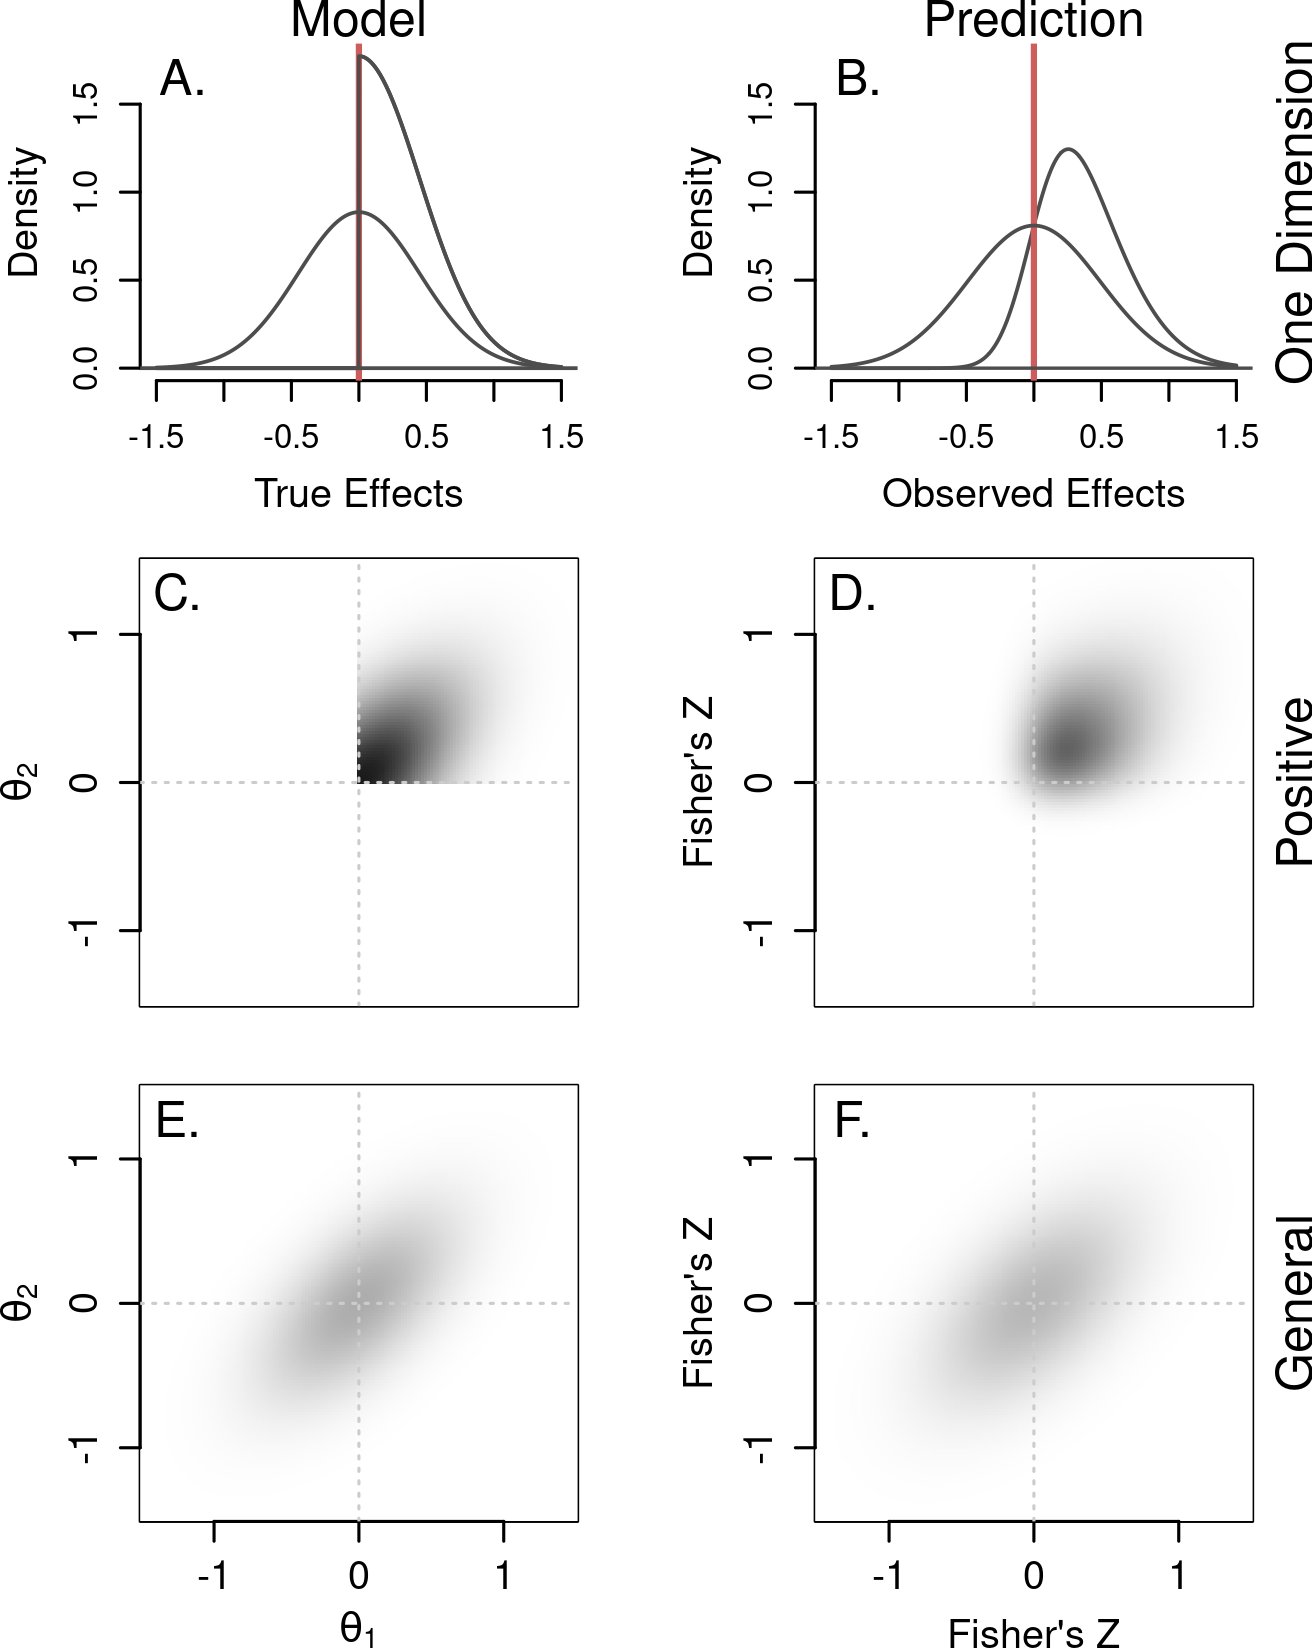
\includegraphics{p_files/figure-latex/meta-modelcomp-1.png}
\caption{\label{fig:meta-modelcomp}Model specification and predictions for the positive-effects model and the general model. The models are on the left hand-side, and the predictions for data are on the right hand-side. Top row: Models for one study. Even though the positive-effects model is restricted to positive values in specification, it can predict small negative observed values. Middle row: Positive-effects model for two studies. Effects for any two studies are predicted to be correlated due to the hiearchical nature of the model, and mostly positive. Bottom row: General model for two studies. Effects are still correlated, but may be positive or negative. The predictions for any specific effect combination is weaker for the general model as is covers more parameter space.}
\end{figure}

In Bayesian model comparison, the main target of interest is the relative evidence for one model compared to another. The Bayes factor is this relative evidence, and it results directly from Bayes rule. We may also view the Bayes factor as \emph{predictive accuracy} of one model over another model (Rouder \& Morey, 2019). In this sense, the Bayes factor denotes how well the first model predicted the observed data compared to the other model. Figure~\ref{fig:meta-modelcomp} illustrates this point. Panel A shows the model specifications for the positive-effects and the unconstrained model for any one study's true effect. The predictions for observed effect sizes from these models are illustrated in panel B. As can be seen, the positive-effects model best predicts positive effects while the general model predicts both positive and negative effects to the same degree. As a result, if a positive effect is observed, the positive-effects model will be preferred as it has more density for positive effects than the general model. In contrast, if a negative effect is observed the general model will be preferred. Yet, the positive-effects model \emph{can} predict small negative effects despite the ordinal constraint on true effects.

How do the model predictions extend to more than one study effect? Figure~\ref{fig:meta-modelcomp} shows multivariate model specifications for two studies for both the unconstrained and the positive-effects model. Panels C and D show model specification and model prediction for the positive-effects model. The effect size for Study 1 is specified on the x-axis; the effect size for Study 2 is specified on the y-axis. The correlation between the two effects is introduced by the hierarchical nature of the models (i.e.~the common variability of the mean effect). This correlation is also preserved in the predictions, and the positive-effects model best predicts small, similar, positive effects. The predictions of the unconstrained model are shown in Figure~\ref{fig:meta-modelcomp}F. Conceptually, Bayes factors can be understood as a comparison between the prediction in panels D and F in Figure~\ref{fig:meta-modelcomp}. If we observed effects for the two studies, say \(z_1 = .2\) and \(z_2 = .25\), then we may compare the predictive accuracy for the point \([.2, .25]\) of these two panels. The ratio of the predictive accuracies at the observed data point is the Bayes factor between the two models.

Practically, Bayes factors can be estimated in several ways. Here, we use the encompassing approach to estimate the Bayes factor between the unconstrained model and the positive-effects model (Haaf \& Rouder, 2017; Hoijtink, 2012; Klugkist, Laudy, \& Hoijtink, 2005), and an analytic approach to assess the Bayes factor between the unconstrained model, the common-effect model, and the null model (Rouder, Morey, Speckman, \& Province, 2012). The Bayes factors between the positive-effects model, the common-effect model, and the null model can be obtained using the transitivity property of Bayes factors.\footnote{Using transitivity, the Bayes factor between the positive-effects model and the null model, \(B_{+0}\), may be obtained as \(B_{+0} = \frac{B_{g0}}{B_{g+}}\).}

The encompassing approach employed here is based on Hoijtink (2012), and we have employed and described the approach in Haaf and Rouder (2017), Haaf and Rouder (2019), and Rouder et al. (2019). More interesting is the analytic approach employed here. Because we use surface statistics (such as Fisher's \(Z\)) and their standard errors as data, we derived the analytic Bayes factor between the unconstrained model and the common-effect model, and between the unconstrained model and the null model from scratch. The main target of the approach is the probability of data conditional on each of the two models marginalized over the parameter space. This probability is typically called the marginal probability of a model, and it may be expressed using The Law of Total Probability as
\begin{equation} \label{eq:bfInt}
P(\bm Y\mid {\cal M}) = \int_{\bm \xi\in \Xi} P(\bm Y|\bm \xi)P(\bm \xi)d\bm \xi,
\end{equation}
where \(\bm \xi\) is a vector of parameters from parameter space \(\Xi\). The likelihood function, \(P(\bm Y|\bm \xi)\), is given by Equation~\eqref{eq:basemodel}, and it is the product of normal densities with mean \(\theta_i\) and variance \(\frac{1}{n_i - 3}\) evaluated for the data.

Here, we illustrate the analytic approach for obtaining the Bayes factor between the null model and the unconstrained model. For the null model, obtaining the marginal probability is straight-forward. The parameter space of \(\theta_i\) is reduced to a vector of zeros. The integral in Equation \eqref{eq:bfInt} is simply the likelihood of the data when \(\theta_i = 0\) for all \(i\). For the unconstrained model, the integral in Equation \eqref{eq:bfInt} may be simplified by integrating out the collection of \(\theta_i\) and the overall effect \(\mu\). The likelihood of \(Z_i\) marginal over \(\theta_i\) and \(\mu\) is

\[Z_i | \tau^2, \sigma^2_\mu \sim \mbox{Normal}(0, \frac{1}{n_i - 3} + \tau^2 + \sigma^2_\mu),\]

where \(\tau^2\) is the variance of \(\theta_i\) and \(\sigma^2_\mu\), the variance of \(\mu\) that is here fixed at \(.15^2\). The integral is now reduced to the dimension of \(\tau^2\). To estimate \(P(\bm Y\mid {\cal M})\) the integral can be evaluated for possible values of \(\tau^2\) based on its prior distribution. The marginal probability can be estimated in similar fashion for the common-effect model.

\hypertarget{application-the-familiar-word-recognition-effect}{%
\section{Application: The Familiar-word-recognition Effect}\label{application-the-familiar-word-recognition-effect}}

\begin{figure}
\centering
\includegraphics{p_files/figure-latex/resFig-1.pdf}
\caption{\label{fig:resFig}Results for the familiar-word-recognition effect from the unconstrained model. Observed effects with 95\% confidence intervals are depicted by the gray squares and bars, posterior estimates with 95\% credible intervals are given by the black points and bars. There is hierarchical shrinkage to the overall effect reducing the variability of study effects drastically.}
\end{figure}

We are now ready to apply the does-everyone meta-analysis to data. Here, we re-analyzed the meta-analysis on the familiar-word-recognition-effect conducted by Carbajal et al. (2020). The authors gathered 34 studies from 16 research articles studying infants with average sample age ranging from 5 to 15 months. Here, null, positive, and negative effects correspond to different stages in early language development (Hallé \& Boysson-Bardies, 1994). If infants do not distinguish between familiar and unfamiliar words then the familiar-word-recognition effect is zero. If infants pay more attention to familiar words than novel ones then the familiar-word-recognition effect is positive. If infants pay more attention to novel words than familiar words then the familiar-word-recognition effect is negative. The expectation is that infants in the age range of the current studies show a positive familiar-word recognition effect. The analysis by Carbajal et al. (2020) showed an overall effect size in line with this expectation, \(\hat{\mu} = 0.21\), \(95\%\)CI \(= [0.13, 0.3]\). Yet, do all studies plausibly show a qualitatively similar effect, that is, is there one underlying phenomenology?

We first estimated the unconstrained model. The observed and estimated study effect sizes (Fisher's \(Z\)) are shown in Figure~\ref{fig:resFig}. The gray squares correspond to the observed effect sizes, and the black points correspond to the estimates from the unconstrained model (posterior means). The gray error bars show the 95\% confidence intervals for Fisher's \(Z\). The black error bars show 95\% credible intervals. The size of the points is determined by the study weights that are in turn dependent on the sample size. These weights determine the impact of each study on the overall effect size. As can be seen, there is a substantial amount of hierarchical shrinkage reducing the variability of estimated study effects as compared to observed study effects. The amount of shrinkage for each study is a function of the standard error of the effect size estimate, which in turn is a function of the sample size. Because the studies in the current meta-analysis have relatively small sample sizes---between 12 and 53 participants---as is typical for developmental research, much hierarchical shrinkage is expected towards the overall effect.

Figure~\ref{fig:resFig} also shows that while three studies have an observed negative effect size the posterior means for all 34 studies are positive. To quantify the evidence for or against every-study-does, we compare the models previously proposed using Bayes factors. The preferred model is the positive-effects model, and it is preferred over the common-effect model by 0 to 1, over the null model by 0 to 1, and over the unconstrained model by 0 to 1 (see Table~\ref{tab:covariate-tab}). Hence, while there is some evidence that all studies show a positive effect, there is only modest evidence that study effects actually differ in true value.

In summary, at this point, it seems that all studies conform with the expectation that infants pay more attention to novel words. Hence, we may tentatively hold onto the notion that all studies are indeed tapping the same psychological processes and belong functionally to a common phenomenology. We find relatively small differences across estimated true effects. Given the common phenomenology we now feel confident to interpret the overall effect across studies, estimated as \(\hat{\mu} \mid \bm Z= 0.20\), \(95\%\)CrI \(= [0.12, 0.29]\). This estimate can be used to inform the design of future studies.

\hypertarget{accounting-for-predictors}{%
\section{Accounting for Predictors}\label{accounting-for-predictors}}

A key goal in meta-analysis is to assess the relationship between a predictor variable and the effect size of a dependent measure across studies (Borenstein, Hedges, Higgins, \& Rothstein, 2011). This goal is especially relevant when there is substantial variability of effect sizes. The hope then is that this variability can be explained by one or more predictors. In the usual case, the researcher is concerned about the effect of the predictor on the meta-analytic mean, and fairly straightforward extensions of linear regression may be used to assess whether a predictor accounts for substantial variability. The consideration of predictors, however, is far more nuanced in a does-every-study framework.

In meta-analysis, it is common to consider predictors that act on what we call \emph{the study level}. These predictors apply to the study as a whole. Examples could be elements of the experimental design, choice of dependent variable, the age of the target population, or the language of the participants. In keeping with the theme of the development, models are specified for the case where researchers have summary-level data for each study and the values of the predictors for each study.

There are two main targets of inquiry: (a) is the inclusion of a predictor warranted, and (b) if so, does the inclusion change whether there are qualitative or quantitative differences in the set of studies. The main approach here is to specify a set of models that encompass these targets and compare them with Bayes factors.

\hypertarget{meta-regression-models}{%
\subsection{Meta-regression Models}\label{meta-regression-models}}

The meta-regression model for a single predictor is:

\begin{align} \label{eq:pred}
Z_i &\sim \mbox{Normal}(\theta_i, \frac{1}{N_i - 3}),\\
\theta_i &= \nu_i + x_i \beta,
\end{align}

where \(x_i\) denotes the predictor for the \(i\)th study, and \(\beta\) denotes the slope. The parameter \(\theta_i\) serves the same role in the previous models without a predictor. To avoid identifiability issues, without any loss of generality we normalize the collection of \(x_i\) such that the mean is zero and the variance is 1. Note that in this model, the parameter \(\nu_i\) combines both a non-zero intercept and residuals. It is not a classic intercept parameter inasmuch as there is one such parameter for each study. It is not a classic residual as it is not zero-centered. The reason for this specification is simple---the model reduces to the previous unconstrained model without predictors when the slope parameter, \(\beta\) is zero. Hence, it is a proper generalization of the previous development. With the understanding that the collection of \(\nu\)s is not zero-centered, we will refer to them as the residuals.

Priors are needed on \(\beta\) and the collection of \(\nu_i\)s. For \(\beta\) we chose a weakly informative, zero-centered prior:
\[\beta \sim \mbox{Normal}(0, 0.15^2).\]
For \(\nu_i\) we kept the prior structure previously shown in the Section \enquote{Prior Settings}:

\begin{align*}
\nu_i &\sim \mbox{Normal}(\mu, \tau^2),\\
\mu &\sim \mbox{Normal}(0, 0.15^2),\\
\tau^2 &\sim \mbox{Inverse-Gamma}(1, 0.02).
\end{align*}

\hypertarget{submodels-and-interpretations}{%
\subsection{Submodels and Interpretations}\label{submodels-and-interpretations}}

The critical question is on the placement of order constraints. In the previous section, we discussed four different models on the true study effects---all were null, all were constant, all were positive, and a lack of constraint. In the regression model, a comparable target is the parameter \(\nu_i\), the residual effect \emph{after} accounting for the predictor. To indicate these models, we extend the previous notation as follows. The model \({\cal M}_{0+\beta}\) is a null model where the predictor is included and the residuals at the study level are all zero. The models \({\cal M}_{c+\beta}\), \({\cal M}_{p+\beta}\), and \({\cal M}_{u+\beta}\), the common residuals, positive residuals, and unconstrained residuals models, are defined likewise. Note that some of these models are much more plausible than others. For example, a model where all residuals are identically zero seems unreasonable. Therefore, we carry the two models we consider most plausible and informative, \({\cal M}_{p+\beta}\) and \({\cal M}_{u+\beta}\).

These regression models are defined by constraint on the residuals. Yet, we can also place constraint on the marginal or total effect, \(\theta_i\). And, surprisingly, the constraint on the marginals and on the residuals may have different implications. The following cases highlight the differences and their theoretical interpretation:

\begin{enumerate}
\def\labelenumi{\roman{enumi}.}
\item
  \emph{Explaining Qualitative Differences.} Consider the case where the total effect \(\theta_i\) violates the positive constraints, that is, there is evidence that at least some \(\theta_i\) are negative. Here, we may conclude that the phenomenon is complex and disunified. Now, suppose that when the predictor is added, the resulting residuals, \(\nu_i\), obey positive constraints. In this case, the rich results in the total is explained by the predictor. That is, the predictor resulted in converting qualitative differences among the studies to quantitative ones. This case, in our view, represents an advancement of knowledge---the predictor clearly explains why some studies are positive and others are negative.
\item
  \emph{Robust Quantitative Differences.} One facet of inference with Bayes factor is that it is calibrated by the resolution of the data (Rouder, Speckman, Sun, Morey, \& Iverson, 2009). When the data are noisy or few in number, simpler models are supported over more complicated ones. In the context of this report, the null model is simplest, followed in order by the common model, the positive model, and the unconstrained model. Adding a predictor that accounts for noise effectively increases the resolution of the data. In some cases, if the predictor is added, it may account for variation, and the net result is that the data now have the resolution to support more complex models, say there is evidence for violations of constraint on the residuals that was previously unavailable. Perhaps even more importantly, the same constraint that was obeyed in the total may still hold when predictors are added. If there is still evidence that all studies show a true positive effect, then every-study-does holds even in light of increased resolution. The constraint is robust to the predictor.
\end{enumerate}

We expand the notation as follows. The model where there is constraint on residuals \(\nu_i\) but not on totals \(\theta_i\) are denoted as above. The models where there is constraint on \(\theta_i\) are indicated with parentheses as follows. The model \({\cal M}_{(p+\beta)_p}\) denotes the constraints where both \(\theta_i\) and \(\nu_i\) are positive. To see if the finding is robust to the covariate, we may check that \({\cal M}_{(p+\beta)_p}\) is superior to all other models. For example, to \({\cal M}_{(p+\beta)_u}\), where with increased resolution from the covariate, we observe violations in the positivity of the marginals. Note that \({\cal M}_{(p+\beta)_u}\) and \({\cal M}_{p+\beta}\) are the same model as they have a constraint on the residuals but not the marginals.

\hypertarget{the-familiar-word-recognition-example}{%
\subsection{The Familiar-word-recognition Example}\label{the-familiar-word-recognition-example}}

For the familiar-word-recognition meta-analysis, we assess the effect of the average age of study samples on the effect size. To do so, we standardize age and estimate the model using Gibbs sampling. Figure~\ref{fig:resfig-cont}A comes from the previous analysis where there is no predictor. One of the things we can see here is shrinkage to the grand mean. Figure~\ref{fig:resfig-cont}B now shows estimates for the meta-regression model with the predictor included. The gray open points again reference the observed effect sizes, and the blue points are the estimates for \(\theta_i\) from the model including the predictor. Notice that the pattern of shrinkage is different: Observed effects are shrunken towards the regression line instead of the grand mean. The slope of the estimated regression line is \(\beta = 0.06\), 95\%CI \(= [-0.03, 0.14]\). This slope is slightly reduced from the least square error regression line (dashed line). This reduction is due to hierarchical shrinkage of study effect sizes.

\begin{figure}
\centering
\includegraphics{p_files/figure-latex/resfig-cont-1.pdf}
\caption{\label{fig:resfig-cont}Comparison of the meta-regression and the intercept-only analysis of age. The x-axes show the standardized average age per study, the y-axes show Fisher's Z effect size estimates. Gray open points are observed effect sizes; blue points are estimated effect sizes from the Bayesian models. A. Results for the intercept-only model. The dashed line corresponds to the average observed effect size; the blue line corresponds to the estimated mean from the Bayesian model. B. Results for the meta-regression model. The dashed line corresponds to a simple least squares regression line; the blue line corresponds to the estimated regression line from the Bayesian meta-regression model. The red dashed line and points denote \(x_i\beta\), the red vertical lines denote the non-zero-centered residuals \(\nu_i\).}
\end{figure}

Figure \ref{fig:resfig-cont}B shows the effect of the predictor on the marginal estimates of the effect. But it does not indicate whether the predictor is evidenced. For that Bayes factors are needed. Table~\ref{tab:covariate-tab} shows Bayes factors for all models as compared to the unconstrained model. As a reminder, \({\cal M}_{u+\beta}\) refers to the model with predictor with no ordinal constraints; \({\cal M}_{p+\beta}\) refers to the model where all residuals, \(\nu_i\), are constrained to be positive; and \({\cal M}_{(p+\beta)p}\) refers to the model were in addition the marginal study effects, \(\theta_i\) are constrained to be positive with the predictor taken into account. Figure \ref{fig:resfig-cont}B highlights the distinction between the latter two models: The dashed line is \(x_i\beta\), the standardized regression line, and the red lines represent \(\nu_i\) for each study. To compare \({\cal M}_{u+\beta}\) and \({\cal M}_{p+\beta}\), we assess if all red lines go upward from the dashed line, that is, if all \(\nu_i > 0\). To compare \({\cal M}_{p+\beta}\) and \({\cal M}_{(p+\beta)p}\) we additionally assess if all blue points, the marginal study effects, are positive, that is, if all \(\theta_i > 0\).

The Bayes factor analysis shows that the preferred model remains the positive-effects model without predictor. Model \({\cal M}_{u+\beta}\), performs poorest with a Bayes factor of 58.49-to-one in favor of the positive-effects model. Model \({\cal M}_{(p+\beta)p}\), on the other hand, is the third-best model after the positive-effects and the common-effect models, with a Bayes factor of 8.69-to-one in favor of the positive-effects model. We note that the best-performing model remains the positive-effects model. Hence, there is no evidence for the need to add the predictor.

\begin{table}[tbp]

\begin{center}
\begin{threeparttable}

\caption{\label{tab:covariate-tab}Bayes factors for the familiar-word-recognition meta-analysis.}

\begin{tabular}{ll}
\toprule
Model & \multicolumn{1}{c}{Bayes factor}\\
\midrule
${\cal M}_{u+\beta}$ & 0.27\\
${\cal M}_{p+\beta}$ & 4.26\\
${\cal M}_{(p+\beta)p}$ & 1.8\\
${\cal M}_{u}*$ & 1\\
${\cal M}_{p}$ & 15.67\\
${\cal M}_{c}$ & 5.27\\
${\cal M}_{0}$ & 1.69\\
\bottomrule
\addlinespace
\end{tabular}

\begin{tablenotes}[para]
\normalsize{\textit{Note.} Bayes factors are in comparison to the unconstrained model.}
\end{tablenotes}

\end{threeparttable}
\end{center}

\end{table}

\hypertarget{critical-predictors}{%
\section{Critical Predictors}\label{critical-predictors}}

As the replication crisis has roiled psychology, there have been a number of prominent failures to replicate previously established results (e.g.~Open Science Collaboration, 2015; Ebersole et al., 2016). One popular set of beliefs is that the original results are in error, that is, the effects in question do not exist. But another popular set of beliefs is that perhaps both sets of results are correct---that is, the original results correctly showed an effect and the replications correctly showed a lack of one. The argument is that there must be some critical differences in the studies---critical hidden predictors that explain when the effect occurs and when it does not (Monin et al., 2014). The goal then is to find the missing critical predictors.

We are not fans of this approach, and were predisposed to think it is a waste of time. Nonetheless, the does-every-study approach with predictors may be easily adapted to assess the conjecture that a critical predictor explains effects and their failures on a study-by-study basis. In the following we develop the model for the conjecture. Then, we apply it to the familiar-word-recognition example for a predictor that the original authors speculated explained the effect. To our surprise, indeed, this predictor is critical and explains when the effect occurs and when it does not. Unfortunately, the unavoidable conclusion is that the effect may merely be an artifact of publication bias.

\hypertarget{the-critical-predictor-some-studies-model}{%
\subsection{The Critical Predictor Some-studies Model}\label{the-critical-predictor-some-studies-model}}

For this approach we ask whether a categorical variable predicts whether a study has a positive effect, or, alternatively, no effect at all. For example, we may want to assess the effect of preregistration on effect size under the hypothesis that preregistered studies have no effect and unregistered studies have an effect. Alternatively, we might think that there is an effect for one experimental procedure but not for the other. We refer to this setup as a \emph{some-studies} model, and in it the categorical variable is manifest.

\begin{figure}
\centering
\includegraphics{p_files/figure-latex/figModerator-1.pdf}
\caption{\label{fig:figModerator}Estimates for the covariate model with study type as some-studies covariate. The black points show estimated study effects from the model where some studies have a zero effect as predicted by the moderator (familiar-word-recognition effect as baseline) and some studies have positive effects as predicted by the moderator (familiar-word-recognition effect as main target of interest). For two studies (Bywater, 2004) the moderator was not reported.}
\end{figure}

With the base model from Equation~\eqref{eq:basemodel} the some-studies model can be placed on \(\theta_i\):

\[
\begin{array}{llr}
{\cal M}_{ss}: && \begin{cases}
\theta_i \stackrel{iid}{\sim} \mbox{Normal}^+(\mu,\tau^2) \quad \mbox{if} \; x_i = 1,\\
\theta_i = 0 \quad \quad \quad \quad \quad \quad \quad \; \mbox{if} \; x_i = 0.
\end{cases}
\end{array}
\]

where \(x_i\) is an indicator variable for the dichotomous predictor at hand. Note that this model is quite constrained: Not only does it predict the direction of the effect for some studies, it also predicts zero-effects for other studies, and it \emph{a priori} assigns each study to either of the two categories.

In the meta-analysis of familiar-word-recognition we consider a predictor called \emph{study use}. Study use refers to whether the familiar-word-recognition effect was used as the target of study or as a baseline when exploring another effect. Through correspondence the original authors (Carbajal et al., 2020) hypothesized that, because data collection in developmental psychology is costly, the data were published irrespective of the outcome if the familiar-word-recognition effect was the target of interest. Conversely, if the effect was considered a baseline it would perhaps be omitted from publication if the outcome was a null finding. As a result, the familiar-word-recognition effect may be inflated for studies where it was considered a baseline effect. We test Carbajal et al.'s conjecture here.

Figure~\ref{fig:figModerator} shows effect size estimates from the model for 32 of the 34 studies where it was clear whether the familiar-word-recognition effect was either target or baseline. In the majority of the studies with small effects the familiar-word-recognition effect was the main target of interest; in the majority of the studies with larger effects the familiar-word-recognition effect was the baseline. We compared the some-studies model with the models from the previous sections using Bayes factors (See Table~\ref{tab:ss-tab}).\footnote{The Bayes factors for the models shown both in Table 1 and Table~\ref{tab:ss-tab} deviate slightly because less studies are included for Table~\ref{tab:ss-tab}.} In accordance with Carbajal et al.'s conjecture, the some-studies model outperforms all the other models, and it is preferred to the positive-effects model by about 11 to 1.

\begin{table}[tbp]

\begin{center}
\begin{threeparttable}

\caption{\label{tab:ss-tab}Bayes factors for the target vs. baseline study analysis.}

\begin{tabular}{ll}
\toprule
Model & \multicolumn{1}{c}{Bayes factor}\\
\midrule
${\cal M}_{u}*$ & 1\\
${\cal M}_{ss}$ & 141.31\\
${\cal M}_{p}$ & 13.37\\
${\cal M}_{c}$ & 5.64\\
${\cal M}_{0}$ & 2.31\\
\bottomrule
\addlinespace
\end{tabular}

\begin{tablenotes}[para]
\normalsize{\textit{Note.} Bayes factors are in comparison to the unconstrained model.}
\end{tablenotes}

\end{threeparttable}
\end{center}

\end{table}

\hypertarget{software}{%
\section{Software}\label{software}}

The analyses presented here are conducted in \texttt{R} (R Core Team, 2016).\footnote{The following packages were used: R (Version 4.0.2; R Core Team, 2016) and the R-packages \emph{abind} (Version 1.4.5; Plate \& Heiberger, 2016), \emph{BayesFactor} (Version 0.9.12.4.2; Morey \& Rouder, 2018), \emph{circular} (Version 0.4.93; Agostinelli \& Lund, 2017), \emph{coda} (Version 0.19.3; Plummer, Best, Cowles, \& Vines, 2006), \emph{fields} (Version 10.3; Douglas Nychka, Reinhard Furrer, John Paige, \& Stephan Sain, 2017), \emph{ggplot2} (Version 3.3.2; Wickham, 2016), \emph{knitr} (Version 1.29; Xie, 2015), \emph{magrittr} (Version 1.5; Bache \& Wickham, 2014), \emph{MASS} (Version 7.3.52; Venables \& Ripley, 2002), \emph{Matrix} (Version 1.2.18; Bates \& Maechler, 2018), \emph{MCMCpack} (Version 1.4.8; Martin, Quinn, \& Park, 2011), \emph{metafor} (Version 2.4.0; Viechtbauer, 2010), \emph{msm} (Version 1.6.8; Jackson, 2011), \emph{mvtnorm} (Version 1.1.1; Genz \& Bretz, 2009; Wilhelm \& G, 2015), \emph{papaja} (Version 0.1.0.9997; Aust \& Barth, 2017), \emph{psych} (Version 1.9.12.31; Revelle, 2018), \emph{scam} (Version 1.2.6; Pya, 2020), \emph{spatialfil} (Version 0.15; Dinapoli \& Gatta, 2015), \emph{tmvtnorm} (Version 1.4.10; Wilhelm \& G, 2015), and \emph{truncdist} (Version 1.0.2; Novomestky \& Nadarajah, 2016).} As we hope this development is attractive to many researchers we took the following steps to make the adoption convenient. First, we provide an \texttt{R}-script containing all necessary functions to compute posterior estimates and Bayes factors at \href{https://github.com/jstbcs/meta-poor/blob/public/share/lib.R}{github}. Second, we developed the Gibbs sampling functions that can be used on new data.\footnote{Some of the analyses provided here are also supported by the \texttt{R}-package \texttt{metaBMA} (Heck, Gronau, \& Wagenmakers, 2019).} The posterior distribution for models without predictors are estimated using the function \texttt{mcmc\_unconstrained()}; the posterior distribution for models with predictors are estimated using the function \texttt{mcmc\_predictor()}; and the posterior distribution for models without critical predictors are estimated using the function \texttt{mcmc\_somesstudies()}. Functions \texttt{get.bfs.ss()} and \texttt{get.bfs.cont()} provide Bayes factor estimation for all proposed models. The analysis of the familiar-word-recognition effect (Carbajal et al., 2020) is provided at \href{https://github.com/jstbcs/meta-poor/blob/public/papers/submission/analysis/analysis_carbajal.Rmd}{github} as well.

\hypertarget{prior-sensitivity}{%
\section{Prior Sensitivity}\label{prior-sensitivity}}

Bayes factor model comparison requires the choice of settings on prior distributions. Some prior settings have minimal influence on the results of the analysis while others have substantial influence. In the current analysis the settings of \(c_1\) and \(c_2\) have the largest influence. One way of assessing the effect of the prior choices on inference is to conduct a sensitivity analyses. In a sensitivity analysis, prior settings are adjusted within reasonable ranges and the resulting variability of Bayes factors is assessed (e.g., Haaf \& Rouder, 2017; Heycke, Gehrmann, Haaf, \& Stahl, 2018). Here, we conduct a sensitivity analysis for the familiar-word-recognition effect. We chose to double and halve the scale on \(\mu\), \(c_1\), and the scale on \(\tau\), \(c_2\) from our original setting (between 0.08 and 0.30).

\begin{table}[tbp]

\begin{center}
\begin{threeparttable}

\caption{\label{tab:tabsens}Prior sensitivity analysis.}

\begin{tabular}{llllll}
\toprule
Setting $c_1$ & \multicolumn{1}{c}{Setting $c_2$} & \multicolumn{1}{c}{$BF_{ssu}$} & \multicolumn{1}{c}{$BF_{ssp}$} & \multicolumn{1}{c}{$BF_{ssc}$} & \multicolumn{1}{c}{$BF_{ss0}$}\\
\midrule
0.15 & 0.15 & 141.31 & 10.57 & 25.04 & 61.30\\
0.30 & 0.30 & 4,527.52 & 908.46 & 102.30 & 15.94\\
0.08 & 0.30 & 419.63 & 121.43 & 117.09 & 18.24\\
0.30 & 0.08 & 2,182.60 & 3.58 & 137.34 & 345.19\\
0.08 & 0.08 & 35.98 & 1.89 & 15.58 & 39.17\\
\bottomrule
\end{tabular}

\end{threeparttable}
\end{center}

\end{table}

Table~\ref{tab:tabsens} shows the Bayes factors for the original analysis (top row) and four additional analyses with varied settings. Bayes factors are between the preferred some-studies model and the unconstrained, positive-effects, common-effect, and null models, respectively. If all values in a row remain above 1 it implies that the some-studies model is superior for the particular prior setting. However, if a values is below 1 it implies that an alternative model is superior, and therefore the inference is not robust to the chosen prior settings. For the data at hand, while Bayes factors vary considerably, the some-studies model is preferred for all settings in the sensitivity analysis. The pattern of Bayes factors is fairly straight-forward: For smaller scale settings the Bayes factor between the positive-effects model and the some-studies model is relatively close to 1; for larger scales the null model is actually preferred over the positive-effects model, and this phenomenon is well-understood as Lindley's paradox (Lindley, 1957). Yet, within these reasonable ranges of prior settings, the some-studies model is robustly preferred over all of its alternatives.

\hypertarget{discussion}{%
\section{Discussion}\label{discussion}}

Meta-analysis is a powerful tool to summarize evidence across several studies. In the absence of the raw data it is the most straight-forward method to combine quantitative results across multiple studies. Here, we address the fundamental issue in meta-analysis of what forms an appropriate summary across studies. Rather than focusing on an overall effect size, we ask whether every study in the data set plausibly shows an effect in the expected direction. The current approach is motivated by the presence of coarse theory in psychology and the desire for robustness and replicability across many design elements. When theory is coarse, it provides at most an ordinal prediction on effects (Haaf et al., 2019). If all studies plausibly show a true effect in the same direction, then the phenomenon may robustly be found across varying operationalizations and study settings. To answer the question whether every study shows a true effect in the same direction we develop a set of models: A general model much like the conventional meta-analytic random-effects model; a positive-effects model where all studies have a true effect in the same direction; a common-effect model where all true effects are the same; and a null model where all true effects are identically zero. To assess the relative strength of evidence between these models, we propose a Bayes factor model comparison approach adapted from Haaf and Rouder (2017) and Rouder et al. (2019). The crucial innovation here is that the new approach takes summary statistics from each study instead of raw data.

A second scientific question for meta-analysis concerns the role of predictor variables. We develop a new set of models that describe how covariates affect the direction of effects. We apply the does-every-study meta-analysis to the familiar-word-recognition effect (Carbajal et al., 2020) in babies. In developmental research, small sample sizes are common, and meta-analysis therefore remains a central methodological approach. The results from our analysis provide evidence for the claim that studies either show a true positive effect, or truly no effect whatsoever. We did not find a qualitative interaction where some studies truly show an opposite effect. Importantly, there seems to be a critical predictor that determines whether a study will show an effect or not. Studies designed to test the effect result in null effects. Those that use the effect incidentally show positive effects. We suspect publication bias when the effect is not the target of the study.

\hypertarget{limitations-and-future-directions}{%
\subsection{Limitations and Future Directions}\label{limitations-and-future-directions}}

With every model development come model assumptions that need to be taken into account. The advantage of the current approach is that it only requires surface summary statistics. However, modeling these surface statistics introduces the assumption that the observed within-study variance is the true variance. This assumption is actually common in many linear modeling setups such as the computation of BIC. How good of an assumption it is is simply a function of the size of the sample. With large sample sizes obviously the observed variance is very close to the true one. With smaller studies such as in developmental psychology, however, the true variance might be quite different.

Another limitation of the current approach is that, except in some cases, it does take publication bias into account. Although we use the some-studies approach to identify a critical predictor we speculate that publication bias plays a role without actually modeling it. Yet, publication bias and questionable research practices are intimately tied to the question of the utility of meta-analysis (Carter, Schönbrodt, Hilgard, \& Gervais, 2017; Corker, 2018). If the studies in the meta-analytic set are heavily biased, using them to learn about the population is difficult.

One of the main innovations in meta-analysis is the proposal of models and methods to correct for publication bias (Duval \& Tweedie, 2000; Hedges, 1984; Iyengar \& Greenhouse, 1988; Simonsohn, Nelson, \& Simmons, 2014; Stanley \& Doucouliagos, 2014). One possible extension of the current modeling approach is to model selection effects simultaneously with true effects (Iyengar \& Greenhouse, 1988; Maier, Bartoš, \& Wagenmakers, 2020). In principle, this extension should not be too difficult. Yet, assessing the success of these corrections can be problematic as neither the process of study censorship nor the amount of publication bias are known in any real meta-analytic set (Guan \& Vandekerckhove, 2016). One additional difficulty here is the role of skewness of the distribution of observed effects. In the current approach, skewness comes from an underlying skewed distribution of true effects; in most publication bias correction models, in contrast, skewness reflects the censoring process. While it may be possible to disentangle publication bias and true positive effects by assessing the relationship of sample size and effect size, a robust, general solution remains an open issue.

A third limitation of the current approach concerns the type of predictors considered in the meta-regression analysis. Here, we only developed a framework for study-level predictors. However, it is increasingly common to assess the effect of within-study predictors such as age per study condition, or different dependent variables assessed within the same sample. If such within-study predictors are included, a three-level meta-analysis has to be conducted to account for the within-study dependency (Cheung, 2014; Van den Noortgate, López-López, Marín-Martínez, \& Sánchez-Meca, 2013). One future improvement may be the extension of every-study-does meta-analysis to three-level meta-analysis.

\hypertarget{conclusion}{%
\subsection{Conclusion}\label{conclusion}}

In summary, the current approach allows to investigate questions of ordinal constraint in a meta-analytic setting. We think that answering the does-every-study question is timely and topical. If, indeed, every study shows a true effect in the same, expected direction, maintaining an underlying theory for the target phenomenon seems reasonable. If, however, the ordinal constraint is violated and some studies show true opposite effects, researchers need to investigate the underlying mechanism that lead to this qualitative interaction. These mechanisms may be found in design or population, and the proposed predictor analysis can help understanding the underlying differences.

\newpage

\hypertarget{references}{%
\section{References}\label{references}}

\begingroup
\setlength{\parindent}{-0.5in}
\setlength{\leftskip}{0.5in}

\hypertarget{refs}{}
\leavevmode\hypertarget{ref-R-circular}{}%
Agostinelli, C., \& Lund, U. (2017). \emph{R package \texttt{circular}: Circular statistics (version 0.4-93)}. CA: Department of Environmental Sciences, Informatics; Statistics, Ca' Foscari University, Venice, Italy. UL: Department of Statistics, California Polytechnic State University, San Luis Obispo, California, USA. Retrieved from \url{https://r-forge.r-project.org/projects/circular/}

\leavevmode\hypertarget{ref-R-papaja}{}%
Aust, F., \& Barth, M. (2017). \emph{papaja: Create APA manuscripts with R Markdown}. Retrieved from \url{https://github.com/crsh/papaja}

\leavevmode\hypertarget{ref-R-magrittr}{}%
Bache, S. M., \& Wickham, H. (2014). \emph{Magrittr: A forward-pipe operator for r}. Retrieved from \url{https://CRAN.R-project.org/package=magrittr}

\leavevmode\hypertarget{ref-R-Matrix}{}%
Bates, D., \& Maechler, M. (2018). \emph{Matrix: Sparse and dense matrix classes and methods}. Retrieved from \url{https://CRAN.R-project.org/package=Matrix}

\leavevmode\hypertarget{ref-Borenstein:etal:2011}{}%
Borenstein, M., Hedges, L. V., Higgins, J. P., \& Rothstein, H. R. (2011). \emph{Introduction to meta-analysis}. John Wiley \& Sons.

\leavevmode\hypertarget{ref-Borenstein:etal:2010}{}%
Borenstein, M., Hedges, L. V., Higgins, J., \& Rothstein, H. R. (2010). A basic introduction to fixed-effect and random-effects models for meta-analysis. \emph{Research Synthesis Methods}, \emph{1}(2), 97--111.

\leavevmode\hypertarget{ref-Carbajal:etal:2020}{}%
Carbajal, M. J., Peperkamp, S., \& Tsuji, S. (2020). \emph{A meta-analysis of infants' word-form recognition}.

\leavevmode\hypertarget{ref-Carter:etal:2017}{}%
Carter, E. C., Schönbrodt, F. D., Hilgard, J., \& Gervais, W. M. (2017). \emph{Correcting for bias in psychology: A comparison of meta-analytic methods.} Retrieved from \url{https://osf.io/preprints/psyarxiv/9h3nu/}

\leavevmode\hypertarget{ref-Cheung:2014}{}%
Cheung, M. W.-L. (2014). Modeling dependent effect sizes with three-level meta-analyses: A structural equation modeling approach. \emph{Psychological Methods}, \emph{19}(2), 211--229.

\leavevmode\hypertarget{ref-Corker:2018}{}%
Corker, K. S. (2018). \emph{Strengths and weaknesses of meta-analyses}. Retrieved from \url{https://psyarxiv.com/6gcnm/}

\leavevmode\hypertarget{ref-Corker:etal:2017}{}%
Corker, K. S., Donnellan, M. B., Kim, S. Y., Schwartz, S. J., \& Zamboanga, B. L. (2017). College student samples are not always equivalent: The magnitude of personality differences across colleges and universities. \emph{Journal of Personality}, \emph{85}(2), 123--135.

\leavevmode\hypertarget{ref-R-spatialfil}{}%
Dinapoli, N., \& Gatta, R. (2015). \emph{Spatialfil: Application of 2D convolution kernel filters to matrices or 3D arrays}. Retrieved from \url{https://CRAN.R-project.org/package=spatialfil}

\leavevmode\hypertarget{ref-R-fields}{}%
Douglas Nychka, Reinhard Furrer, John Paige, \& Stephan Sain. (2017). Fields: Tools for spatial data. Boulder, CO, USA: University Corporation for Atmospheric Research. doi:\href{https://doi.org/10.5065/D6W957CT}{10.5065/D6W957CT}

\leavevmode\hypertarget{ref-Duval:Tweedie:2000}{}%
Duval, S., \& Tweedie, R. (2000). Trim and fill: A simple funnel-plot-based method of testing and adjusting for publication bias in meta-analysis. \emph{Biometrics}, \emph{56}, 455--463. Retrieved from \url{10.1111/j.0006-341X.2000.00455.x}

\leavevmode\hypertarget{ref-Ebersole:etal:2016}{}%
Ebersole, C. R., Atherton, O. E., Belanger, A. L., Skulborstad, H. M., Allen, J. M., Banks, J. B., \ldots{} Nosek, B. A. (2016). Many labs 3: Evaluating participant pool quality across the academic semester via replication. \emph{Journal of Experimental Social Psychology}, \emph{67}, 68--82. Retrieved from \url{http://ezid.cdlib.org/id/doi:10.17605/OSF.IO/QGJM5}

\leavevmode\hypertarget{ref-Ferguson:1996}{}%
Ferguson, T. S. (1996). \emph{A course in large sample theory}. Chapman \& Hall Ltd.

\leavevmode\hypertarget{ref-Gail:Simon:1985}{}%
Gail, M., \& Simon, R. (1985). Testing for qualitative interactions between treatment effects and patient subsets. \emph{Biometrics}, \emph{41}(2), 361--372.

\leavevmode\hypertarget{ref-R-mvtnorm}{}%
Genz, A., \& Bretz, F. (2009). \emph{Computation of multivariate normal and t probabilities}. Heidelberg: Springer-Verlag.

\leavevmode\hypertarget{ref-Guan:Vandekerckhove:2016}{}%
Guan, M., \& Vandekerckhove, J. (2016). A Bayesian approach to mitigation of publication bias. \emph{Psychonomic Bulletin and Review}, \emph{23}(1), 74--86. Retrieved from \url{http://www.cidlab.com/prints/guan2015bayesian.pdf}

\leavevmode\hypertarget{ref-Haaf:etal:2019}{}%
Haaf, J. M., Klaassen, F., \& Rouder, J. N. (2019). \emph{Capturing ordinal theoretical constraint in psychological science}. Retrieved from \url{https://psyarxiv.com/a4xu9/}

\leavevmode\hypertarget{ref-Haaf:Rouder:2017}{}%
Haaf, J. M., \& Rouder, J. N. (2017). Developing constraint in Bayesian mixed models. \emph{Psychological Methods}, \emph{22}(4), 779--798.

\leavevmode\hypertarget{ref-Haaf:Rouder:2019}{}%
Haaf, J. M., \& Rouder, J. N. (2019). Some do and some don't? Accounting for variability of individual difference structures. \emph{Psychonomic Bulletin and Review}, \emph{26}, 772--789. Retrieved from \url{https://doi.org/10.3758/s13423-018-1522-x}

\leavevmode\hypertarget{ref-Halle:Boysson:1994}{}%
Hallé, P. A., \& Boysson-Bardies, B. de. (1994). Emergence of an early receptive lexicon: Infants' recognition of words. \emph{Infant Behavior and Development}, \emph{17}(2), 119--129.

\leavevmode\hypertarget{ref-Heck:etal:2019}{}%
Heck, D., Gronau, Q., \& Wagenmakers, E. (2019). \emph{MetaBMA: Bayesian model averaging for random and fixed effects meta-analysis}. Retrieved from \url{https://github.com/danheck/metaBMA}

\leavevmode\hypertarget{ref-Hedges:1984}{}%
Hedges, L. V. (1984). Estimation of effect size under nonrandom sampling: The effects of censoring studies yielding statistically insignificant mean differences. \emph{Journal of Educational Statistics}, \emph{9}(1), 61--85.

\leavevmode\hypertarget{ref-Hedges:Vevea:1998}{}%
Hedges, L. V., \& Vevea, J. L. (1998). Fixed-and random-effects models in meta-analysis. \emph{Psychological Methods}, \emph{3}(4), 486.

\leavevmode\hypertarget{ref-Heycke:etal:2018}{}%
Heycke, T., Gehrmann, S., Haaf, J. M., \& Stahl, C. (2018). Of two minds or one? A registered replication of rydell et al.(2006). \emph{Cognition and Emotion}, \emph{0}(0), 1--20.

\leavevmode\hypertarget{ref-Higgins:etal:2009}{}%
Higgins, J. P., Thompson, S. G., \& Spiegelhalter, D. J. (2009). A re-evaluation of random-effects meta-analysis. \emph{Journal of the Royal Statistical Society: Series A (Statistics in Society)}, \emph{172}(1), 137--159.

\leavevmode\hypertarget{ref-Hoijtink:2012}{}%
Hoijtink, H. (2012). \emph{Informative Hypotheses. Theory and Practice for Behavioral and Social Scientists}. Boca Raton: Chapman \& Hall/CRC.

\leavevmode\hypertarget{ref-Iyengar:Greenhouse:1988}{}%
Iyengar, S., \& Greenhouse, J. B. (1988). Selection models and the file drawer problem. \emph{Statistical Science}, 109--117.

\leavevmode\hypertarget{ref-R-msm}{}%
Jackson, C. H. (2011). Multi-state models for panel data: The msm package for R. \emph{Journal of Statistical Software}, \emph{38}(8), 1--29. Retrieved from \url{http://www.jstatsoft.org/v38/i08/}

\leavevmode\hypertarget{ref-Jeffreys:1961}{}%
Jeffreys, H. (1961). \emph{Theory of probability (3rd edition)}. New York: Oxford University Press.

\leavevmode\hypertarget{ref-Kass:Raftery:1995}{}%
Kass, R. E., \& Raftery, A. E. (1995). Bayes factors. \emph{Journal of the American Statistical Association}, \emph{90}, 773--795. Retrieved from \url{http://amstat.tandfonline.com/doi/abs/10.1080/01621459.1995.10476572}

\leavevmode\hypertarget{ref-Klugkist:etal:2005}{}%
Klugkist, I., Laudy, O., \& Hoijtink, H. (2005). Inequality constrained analysis of variance: A Bayesian approach. \emph{Psychological Methods}, \emph{10}(4), 477.

\leavevmode\hypertarget{ref-Lindley:1957}{}%
Lindley, D. V. (1957). A statistical paradox. \emph{Biometrika}, \emph{44}, 187--192.

\leavevmode\hypertarget{ref-Maier:etal:2020}{}%
Maier, M., Bartoš, F., \& Wagenmakers, E.-J. (2020). Robust bayesian meta-analysis: Addressing publication bias with model-averaging.

\leavevmode\hypertarget{ref-R-MCMCpack}{}%
Martin, A. D., Quinn, K. M., \& Park, J. H. (2011). MCMCpack: Markov chain monte carlo in R. \emph{Journal of Statistical Software}, \emph{42}(9), 22. Retrieved from \url{http://www.jstatsoft.org/v42/i09/}

\leavevmode\hypertarget{ref-Monin:etal:2014}{}%
Monin, B., Oppenheimer, D. M., Ferguson, M. J., Carter, T. J., Hassin, R. R., Crisp, R. J., \ldots{} others. (2014). Commentaries and rejoinder on klein et al.(2014). \emph{Social Psychology}, 299--311.

\leavevmode\hypertarget{ref-Morey:etal:2016}{}%
Morey, R. D., Romeijn, J.-W., \& Rouder, J. N. (2016). The philosophy of Bayes factors and the quantification of statistical evidence. \emph{Journal of Mathematical Psychology}, \emph{72}, 6---18. Retrieved from \url{http://www.sciencedirect.com/science/article/pii/S0022249615000723}

\leavevmode\hypertarget{ref-R-BayesFactor}{}%
Morey, R. D., \& Rouder, J. N. (2018). \emph{BayesFactor: Computation of bayes factors for common designs}. Retrieved from \url{https://CRAN.R-project.org/package=BayesFactor}

\leavevmode\hypertarget{ref-R-truncdist}{}%
Novomestky, F., \& Nadarajah, S. (2016). \emph{Truncdist: Truncated random variables}. Retrieved from \url{https://CRAN.R-project.org/package=truncdist}

\leavevmode\hypertarget{ref-OpenScienceCollaboration:2015}{}%
Open Science Collaboration. (2015). Estimating the reproducibility of psychological science. \emph{Science}, \emph{349}(6521), 943. Retrieved from \href{dx.doi.org/10.1126/science.aac4716\%20}{dx.doi.org/10.1126/science.aac4716 }

\leavevmode\hypertarget{ref-Pan:Wolfe:1997}{}%
Pan, G., \& Wolfe, D. A. (1997). Test for qualitative interaction of clinical significance. \emph{Statistics in Medicine}, \emph{16}(14), 1645--1652.

\leavevmode\hypertarget{ref-R-abind}{}%
Plate, T., \& Heiberger, R. (2016). \emph{Abind: Combine multidimensional arrays}. Retrieved from \url{https://CRAN.R-project.org/package=abind}

\leavevmode\hypertarget{ref-R-coda}{}%
Plummer, M., Best, N., Cowles, K., \& Vines, K. (2006). CODA: Convergence diagnosis and output analysis for mcmc. \emph{R News}, \emph{6}(1), 7--11. Retrieved from \url{https://journal.r-project.org/archive/}

\leavevmode\hypertarget{ref-R-scam}{}%
Pya, N. (2020). \emph{Scam: Shape constrained additive models}. Retrieved from \url{https://CRAN.R-project.org/package=scam}

\leavevmode\hypertarget{ref-R-base}{}%
R Core Team. (2016). \emph{R: A language and environment for statistical computing}. Vienna, Austria: R Foundation for Statistical Computing. Retrieved from \url{https://www.R-project.org/}

\leavevmode\hypertarget{ref-R-psych}{}%
Revelle, W. (2018). \emph{Psych: Procedures for psychological, psychometric, and personality research}. Evanston, Illinois: Northwestern University. Retrieved from \url{https://CRAN.R-project.org/package=psych}

\leavevmode\hypertarget{ref-Rouder:etal:2018}{}%
Rouder, J. N., Haaf, J. M., \& Aust, F. (2018). From theories to models to predictions: A Bayesian model comparison approach. \emph{Communication Monographs}, \emph{85}, 41--56. Retrieved from \url{https://doi.org/10.1080/03637751.2017.1394581}

\leavevmode\hypertarget{ref-Rouder:etal:2019b}{}%
Rouder, J. N., Haaf, J. M., Davis-Stober, C. P., \& Hilgard, J. (2019). Beyond overall effects: A Bayesian approach to finding constraints in meta-analysis. \emph{Psychological Methods}.

\leavevmode\hypertarget{ref-Rouder:Morey:2019}{}%
Rouder, J. N., \& Morey, R. D. (2019). Teaching bayes' theorem: Strength of evidence as predictive accuracy. \emph{The American Statistician}, \emph{73}, 186--190. Retrieved from \url{https://doi.org/10.1080/00031305.2017.1341334}

\leavevmode\hypertarget{ref-Rouder:etal:2012}{}%
Rouder, J. N., Morey, R. D., Speckman, P. L., \& Province, J. M. (2012). Default Bayes factors for ANOVA designs. \emph{Journal of Mathematical Psychology}, \emph{56}, 356--374. Retrieved from \url{http://dx.doi.org/10.1016/j.jmp.2012.08.001}

\leavevmode\hypertarget{ref-Rouder:etal:2016b}{}%
Rouder, J. N., Morey, R. D., \& Wagenmakers, E.-J. (2016). The interplay between subjectivity, statistical practice, and psychological science. \emph{Collabra}, \emph{2}, 6. Retrieved from \url{http://doi.org/10.1525/collabra.28}

\leavevmode\hypertarget{ref-Rouder:etal:2009a}{}%
Rouder, J. N., Speckman, P. L., Sun, D., Morey, R. D., \& Iverson, G. (2009). Bayesian \(t\)-tests for accepting and rejecting the null hypothesis. \emph{Psychonomic Bulletin and Review}, \emph{16}, 225--237. Retrieved from \url{http://dx.doi.org/10.3758/PBR.16.2.225}

\leavevmode\hypertarget{ref-Simonsohn:etal:2014}{}%
Simonsohn, U., Nelson, L. D., \& Simmons, J. P. (2014). P-curve: A key to the file-drawer. \emph{Journal of Experimental Psychology: General}, \emph{143}, 534--547. Retrieved from \url{10.1037/a0033242}

\leavevmode\hypertarget{ref-Stanley:Doucouliagos:2014}{}%
Stanley, T. D., \& Doucouliagos, H. (2014). Meta-regression approximations to reduce publication selection bias. \emph{Research Synthesis Methods}, \emph{5}(1), 60--78. Retrieved from \href{DOI:\%2010.1002/jrsm.1095}{DOI: 10.1002/jrsm.1095}

\leavevmode\hypertarget{ref-VandenNoortgate:etal:2013}{}%
Van den Noortgate, W., López-López, J. A., Marín-Martínez, F., \& Sánchez-Meca, J. (2013). Three-level meta-analysis of dependent effect sizes. \emph{Behavior Research Methods}, \emph{45}(2), 576--594.

\leavevmode\hypertarget{ref-R-MASS}{}%
Venables, W. N., \& Ripley, B. D. (2002). \emph{Modern applied statistics with s} (Fourth.). New York: Springer. Retrieved from \url{http://www.stats.ox.ac.uk/pub/MASS4}

\leavevmode\hypertarget{ref-R-metafor}{}%
Viechtbauer, W. (2010). Conducting meta-analyses in R with the metafor package. \emph{Journal of Statistical Software}, \emph{36}(3), 1--48. Retrieved from \url{http://www.jstatsoft.org/v36/i03/}

\leavevmode\hypertarget{ref-Wagenmakers:etal:2016b}{}%
Wagenmakers, E.-J., Beek, T., Dijkhoff, L., Gronau, Q. F., Acosta, A., R. B. Adams, J., \ldots{} Zwaan, R. A. (2016). Registered replication report: Strack, martin, \& stepper (1988). \emph{Perspectives on Psychological Science}, \emph{11}(6), 917--928. Retrieved from \url{https://doi.org/10.1177/1745691616674458}

\leavevmode\hypertarget{ref-R-ggplot2}{}%
Wickham, H. (2016). \emph{Ggplot2: Elegant graphics for data analysis}. Springer-Verlag New York. Retrieved from \url{http://ggplot2.org}

\leavevmode\hypertarget{ref-R-tmvtnorm}{}%
Wilhelm, S., \& G, M. B. (2015). \emph{tmvtnorm: Truncated multivariate normal and student t distribution}. Retrieved from \url{http://CRAN.R-project.org/package=tmvtnorm}

\leavevmode\hypertarget{ref-R-knitr}{}%
Xie, Y. (2015). \emph{Dynamic documents with R and knitr} (2nd ed.). Boca Raton, Florida: Chapman; Hall/CRC. Retrieved from \url{https://yihui.name/knitr/}

\endgroup

\newpage

\hypertarget{appendix}{%
\section{Appendix}\label{appendix}}

The asymptotic distribution of \(Z\) is well established for the correlation between two independent and identically distributed normal random variables (Ferguson, 1996). In the case of correlation, Fisher's \(Z\) serves as normalized correlation measure. Yet, how does Fisher's \(Z\) translate to experimental data? Let's assume an experimental setup with \(j\) conditions, \(j = 1, 2\). The \(i\)th participant is assigned to one of the two conditions, \(i = 1, \ldots, 2n\), where \(n\) is the number of participants in each condition and \(2n\) is the total number of participants. Then \(Y_i\) denotes the \(i\)th person's observation with

\begin{align}\label{eq:defY}
Y_{i} \sim \begin{cases} \mbox{Normal}(\mu_1, \sigma^2) & \mbox{if } i = 1, \ldots, n,\\
\mbox{Normal}(\mu_2, \sigma^2) & \mbox{if } i = n + 1, \ldots, 2n,\end{cases}
\end{align}

where \(\mu_j\) denotes the true mean of the \(j\)th condition and \(\sigma^2\) denotes the within-group variance. To calculate Fisher's \(Z\) as effect size measure we could first calculate Cohen's \(d\) and then use common transformations via the correlation coefficient \(r\). To understand what this correlation coefficient represents we may define a new variable, \(X_i\), that denotes \(i\)th participant's condition. \(X_i\) is an effect variable encoding \(j = 1\) as \(X_i = -1\) and \(j = 2\) as \(X_i = 1\). The correlation coefficient \(r\) is the point-biserial correlation between \(\mathbf{X}\) and \(\mathbf{Y}\), and Fisher's \(Z\) may be calculated using Equation~\eqref{eq:Zcalc}. Yet, we need to verify that the asymptotic distribution of Fisher's \(Z\) for the biserial correlation is the same as the asymptotic distribution of Fisher's \(Z\) for the bivariate normal. Here, we provide a proof that the asymptotic variance is stable and does not depend on the size of the effect.

Let \(\bar{Y}\) be the grand mean of \(\mathbf{Y}\), \(\bar{Y} = 1/2 (\bar{Y}_1 + \bar{Y}_2)\). Here, \(\bar{Y}_1\) denotes the mean of \(Y_i\) for \(i = 1, \ldots, n\), and \(\bar{Y}_2\) denotes the mean of \(Y_i\) for \(i = n + 1, \ldots, 2n\). Let \(S_{YY}\) denote the variance of \(\mathbf{Y}\), \(S_{YY} = \sum_1^n (Y_i - \bar{Y}_1)^2 + \sum_{n+1}^{2n} ( Y_i - \bar{Y}_2)^2 + n/2 (\bar{Y}_1 - \bar{Y}_2)^2 = SS_1 + SS_2 + n/2 (\bar{Y}_1 - \bar{Y}_2)^2\), where \(SS_1\) is the sum of squares for \(i = 1, \ldots, n\), and \(SS_2\) is the sum of squares for \(i = n + 1, \ldots, 2n\). Let \(S_{XX} = 2n\) denote the variance of \(\mathbf{X}\) and let \(S_{XY} = n(\bar{Y}_1 - \bar{Y}_2)\) denote the covariance of \(\mathbf{X}\) and \(\mathbf{Y}\). We can now insert these quantities into the formula for the correlation coefficient \(r\):

\begin{align*}
r &= \frac{S_{XY}}{\sqrt{S_{XX}S_{YY}}}\\
&= \frac{\sqrt{1/2}(\bar{Y}_1 - \bar{Y}_2)}{\sqrt{\frac{2(SS_1 + SS_2)}{2n} + 1/2(\bar{Y}_1 - \bar{Y}_2)^2)}}.
\end{align*}

We may define a new random variable \(m_n = \bar{Y}_1 - \bar{Y}_2\). Then, based on the Central Limit Theorem:

\[\sqrt{n}(m_n - \Delta) \stackrel{\mathscr{D}}{\rightarrow} \mbox{Normal}(0, 2 \sigma^2),\]

where \(\Delta\) is the true effect. The pooled variance of \(\mathbf{Y}\) is \(S_n = \frac{SS_1 + SS_2}{2n}\).\footnote{Note that \(S_n\) is not the variance of \(\mathbf{Y}\), but the pooled variance of \(Y_i\) if \(i = 1, \ldots, n\) and \(Y_i\) if \(i = n + 1, \ldots, 2n\)} The Central Limit Theorem gives \(\sqrt{n}(S_n - 2\sigma^2) \stackrel{\mathscr{D}}{\rightarrow} \mbox{Normal}(0, 4\sigma^2)\). Using the two asymptotic distributions, \(r \rightarrow \frac{\sqrt{1/2}(\Delta)}{\sqrt{4\sigma^2 + \Delta^2/2}}\). Let \(\Sigma\) be the variance-covariance matrix of \(\big(\begin{smallmatrix} m_n\\ S_n \end{smallmatrix}\big)\):

\[\Sigma = 
\begin{bmatrix}
2\sigma^2 & 0\\
0 & 4\sigma^2
\end{bmatrix}.
\]

And let \(h(a, b) = \frac{\sqrt{1/2}(a)}{\sqrt{2b + a^2/2}}\). The partial derivatives of \(h(a, b)\) are:

\begin{align*}
\frac{\partial h}{\partial a} &= \frac{\sqrt{2} b}{(2b + a^2/2)^{3/2}},\\
\frac{\partial h}{\partial b} &= -\frac{a}{\sqrt{2}(2b + a^2/2)^{3/2}}.
\end{align*}

Using the Delta-method (Ferguson, 1996), we may express the asymptotic distribution of \(h(m_n, S_n)\) as

\[\sqrt{n}(h(m_n, S_n) - h(\Delta, 2\sigma^2) \stackrel{\mathscr{D}}{\rightarrow} \mbox{Normal}(0, \Sigma^*),\]

where \(h(m_n, S_n)\) is the correlation coefficient, the mean, \(h(\Delta, 2\sigma^2)\), is the true correlation coefficient, \(\rho\), and the asymptotic variance is

\begin{align*}
\Sigma^* &= \Big(\frac{2\sqrt{2} \sigma^2}{(4\sigma^2 + \Delta^2/2)^{3/2}}\Big)^2 2\sigma^2 + \Big(\frac{- \Delta}{\sqrt{2}(4\sigma^2 + \Delta^2/2)^{3/2}}\Big)^2 4\sigma^2 \\
&= \frac{16}{\big(8 + \frac{\Delta^2}{\sigma^2}\big)^2}.
\end{align*}

We may apply Fisher's \(Z\) transformation to stabilize the variance. Let \(g(r) = 1/2 \log \big(\frac{1 + r}{1 - r}\big)\). Then \(g'(r) = \frac{1}{1 - r^2}\). Substituting \(h(\Delta, 2\sigma^2)\) for \(\rho\), \(g'(\rho) = \frac{8 + \frac{\Delta^2}{\sigma^2}}{8}\). We may again use the Delta-method to express the asymptotic distribution of \(Z\):

\[\sqrt{n}(g(r) - g(\rho) \stackrel{\mathscr{D}}{\rightarrow} \mbox{Normal}(0, (g'(\rho))^2 \Sigma^*),\]

where \(g(r) = Z\) and \(g(\rho) = \theta\). The asymptotic variance is

\[
(g'(\rho))^2 \Sigma^* = \frac{\cancel{(8 + \frac{\Delta^2}{\sigma^2})^2}}{8^2} \frac{16}{\big(\cancel{8 + \frac{\Delta^2}{\sigma^2}\big)^2}} = 1/4.
\]

Crucially, this value, \(1/4\), does not depend on \(\rho\).


\end{document}
